%------------------------------------------------
%\noindent The specific aims are to:
\begin{comment}
\begin{itemize}
\item[ \textbf{1)}]{
       \textbf{Establish an extensible DWI processing pipeline for large-scale, multicenter brain analysis}
       \newline The development of reliable and valid measurements in brain morphology is important in study of subtle differences in neurodegenerative disorders like Alzheimer's disease, schizophrenia and HD. To study these subtle differences, large samples of subjects from many different data collection sites must be studied. This work aims to develop a DWI processing pipeline, a Nipype wrapped workflow, to perform a volumetric analysis on a large scale heterogeneous diffusion-weighted imaging dataset. This DWI processing pipeline consists of a series of image processing techniques assembled for artifact-correction, alignment, segmentation, compressed sensing, tensors and scalar maps estimation, and statistical measurements. This workflow extents the previous pre-processing steps \cite{Matsui2014} to provide an extensible infrastructure for reliable cross-sectional and longitudinal analysis that allows neuroscientists to measure information about white matter tissues currently inaccessible with standard methods of analysis. This pipeline will be validated on input DWI data from PREDICT-HD dataset.
       %The DWI processing pipeline consists of a series of image processing techniques assembled for artifact-correction, alignment, segmentation, compressed sensing, tensors and scalar maps estimation, and statistical measurements to perform a volumetric analysis on the input diffusion-weighted imaging data from PREDICT-HD dataset. This pipeline extents the previous pre-processing steps \cite{Matsui2014} to provide more reliable cross-sectional and longitudinal analysis for input heterogeneous multi-site DWI data by measuring information about white matter tissue currently inaccessible with standard methods of analysis.
       }
\item[ \textbf{2)}]{
       \textbf{Use complementary information provided by diffusion-weighted imaging data to enhance tissue classification of MR data using a fuzzy k-Nearest Neighbor algorithm}
        \newline Based on the provided pipeline development infrastructure, we show that segmentation quality can be improved for large-scale longitudinal data by incorporating complimentary information acquired from DWI data. 
        }
\item[ \textbf{3)}]{
       \textbf{A novel image registration method that performs consistently on large-scale, multicenter DWI data}
        \newline aaaa
        }
\end{itemize}
\end{comment}
%------------------------------------------------




\section{Specific Aims}
\label{specificAims}
\noindent This research proposes to establish and develop an extensible automated processing pipeline to apply novel cutting-edge methods of \textit{in vivo} diffusion MRI analysis in large-scale multi-center studies. 
\newline
\newline
Diffusion-weighted MR imaging (DWI) is known to be more sensitive to microscopic degeneration than structural MRI. Measuring diffusion properties of functional white matter areas in the time course of their degeneration will help us to advance our understanding of neuropathological basis in neurodegenerative diseases like Huntington's Disease (HD).
\newline
\newline
Therefore, HD will be used as a model here, and the developed methods in this study will be validated on large-scale, multi-site clinical data from PREDICT-HD database \cite{PREDICT_HD}. This dataset contains structural MRI and DWI of brain and a comprehensive set of clinical correlates, that are non-imaging measures including motor and cognitive tests, from a very large sample of individuals with pre-manifest (prodromal) HD, whose HD symptomatology were tracing from its very earliest signs. To combine the strengths of PREDICT-HD dataset with cutting-edge neuroimaging technologies, it is important to have a reliable tool that performs efficiently and consistently for data from many different collection sites.
\newline
\newline
This study uses neuroimaging in python pipelines and interfaces (NIPYPE) to
develop an extensible, automated and reliable processing tool for cross-sectional and longitudinal analysis that allows for non-invasive study of alterations in key brain white matter structures. 
\newline
\newline
First, we investigate the ability of NIPYPE wrapped pipeline to utilize High Performance Computing (HPC) resources to achieve time-efficient data processing and analysis for large-scale study. Then, we propose novel methods that use the complementary information provided by diffusion-weighted imaging data to enhance the classification and registration results previously generated from structural MRI data alone.
\newline

\subsection{Aim 1: Establish an extensible DWI processing pipeline for large-scale, multi-center brain analysis}
The development of reliable and valid measurements in brain morphology is important in study of subtle differences in neurodegenerative disorders like Alzheimer's disease, schizophrenia and HD. To study these subtle differences, large samples of subjects from many different data collection sites must be studied. This work aims to develop a DWI processing pipeline, a NIPYPE wrapped workflow, to perform a volumetric analysis on a large scale heterogeneous diffusion-weighted imaging dataset. This DWI processing pipeline consists of a series of image processing techniques assembled for artifact-correction, alignment, segmentation, compressed sensing, tensors and scalar maps estimation, and statistical measurements. This workflow extents the previous pre-processing steps \cite{Matsui2014} to provide an extensible infrastructure for reliable cross-sectional and longitudinal analysis that allows neuroscientists to measure information about white matter tissues currently inaccessible with standard methods of analysis. This pipeline will be validated on input DWI data from PREDICT-HD dataset.
\newline

\subsection{Aim 2: Use complementary information derived from diffusion-weighted imaging data to enhance tissue classification of MR data}
Based on the developed DWI pipeline infrastructure, we study the improvement of segmentation quality for large-scale multi-site longitudinal MR images by incorporating complimentary information acquired from DWI data.

\subsubsection{Enhance tissue classification by a fuzzy k-Nearest Neighbor classifier using only structural MR data}
\label{MROnlyKNN}
Previous studies on PREDICT-HD dataset have developed a robust multi-modal tool for automated registration, bias correction and tissue classification based on expectation maximization (EM) method \cite{Kim2013}. This task aims to extend the EM-based classification using a non-parametric fuzzy k-Nearest Neighbor classifier that can potentially model more complex decision boundaries than a Gaussian distribution based mixture model.
\newline

\noindent The first task will investigate the probable enhancements using only multimodal structural MR images, all having the same isotropic $1\times1\times1$ $mm^3$ voxel lattice, for training and testing the proposed k-NN method. It is expected that $EM$-based only classification results will be enhanced by the add-on $kNN$ classifier. Then, further potential improvements can be studied using the complementary information derived from diffusion-weighted imaging data processing.

\subsubsection{Incorporate the diffusion derived complementary information to expand the feature space of fuzzy k-NN classifier}
Further potential improvements in tissue classification results will be investigated by incorporating the complementary information acquired from diffusion-weighted imaging data, processed by Aim 1, in to the k-NN classifier infrastructure, developed in section \ref{MROnlyKNN}. For example $FA$ image has a great contrast for white matter regions that can help a better training for the k-NN classifier in a higher order feature space. However, several issues should be tackled before we can incorporate this complementary information into the proposed method, since DWI scans and their post processing derived rotationally invariant scalars (RISs) are in a different voxel space and have lower resolution than their corresponding structural MR T1/T2 scans. This misalignment between voxel sizes and voxel locations causes partial volume effect (PVE) in region boundaries that can result in worse classifications.
\newline

\subsection{Aim 3: Super-resolution of diffusion-weighted images using the anatomical boundaries information}
Accomplishment of enhanced classification methods in Aim 2 will provide better classification results with more reliable tissue boundaries. This task aims to use these boundary curves for the super-resolution reconstruction of low resolution diffusion-weighted imaging data.
The goal is to increase the spatial resolution of DWI scans to a higher resolution isotropic ($1\times1\times1$ $mm^3$) voxel lattice. However, using basic interpolation techniques to resample the input DWI data to a higher resolution voxel space introduces no new information into the input images useful for further medical imaging applications. This study investigates the use of boundary information from isotropic $1\times1\times1$ $mm^3$ posterior tissue probability maps to achieve a super-resolution reconstruction of DWI scans, where the voxel values at tissue boundaries are in agreement with true anatomical definitions in the output image.
\newline
%\subsection{Aim 4: Consistent registration of DWI scans using a multimodal registration framework}








%========================
%pure plugs approach
%========================

\paragraph{Approach} %--------------------------------

Classification accuracy can be improved by excluding the voxels affected by partial volume composition, termed as \textit{mixed samples}, from the initialization of the $EM$ algorithm and the training of the $KNN$ classifier.
In this section, we propose to identify the pure samples by computing a binary mask, called \textbf{pure plugs mask}, that excludes all the mixed samples from the initialization/training of the classification methods.

\subparagraph{What is a pure plug?}
\label{section:purePlugDef}

A \textit{pure plug} is defined as a region (plug), where all multi-modal images have consistent information within the entire range of that region. The size of each plug region is then decided based on the lowest spatial resolution at each direction within all input modality scans.

\subparagraph{Computing a pure plugs mask}

To compute a pure plugs mask, we should avoid both inherent PVE at tissue boundaries and the PVE caused by information inconsistency through multiple modality channels.
Following steps are proposed to compute a pure plugs mask:

\begin{itemize}
\item[ \textbf{1)}]{
       \textbf{Create an empty mask:}
       An empty mask is created to have the lowest spatial resolution at each direction between all input multi-modal scans. All the voxel values are then set to $1$ as a default.
       }
\item[ \textbf{2)}]{
       \textbf{Avoid inherent PVE:}
        All the voxels located in tissue boundaries may include a mixture of both tissue regions, since biology cannot conform in the resolution levels that scanners produce. This inherent partial volume effect is avoided by excluding all tissue boundaries from the pure plugs mask. For this purpose, edges are detected from the input modality with the finest resolution using a Canny edge detector as shown by Figure (\ref{fig:canny_edge_mask}) and are excluded from the default mask created in step (1).
        
%--------------------------------
\begin{figure}
\centering
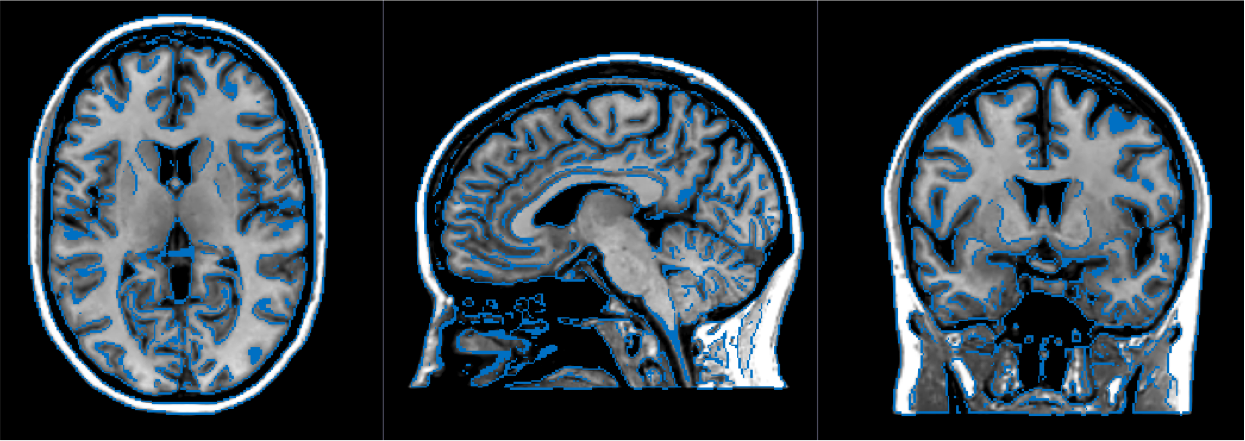
\includegraphics[width=5.5in,height=2in]{canny_edge_mask}\
\centering
\caption{Anatomical tissue boundaries are detected using a Canny edge detector. Detected edges should be excluded from the pure plugs mask to avoid inherent PVE in tissue boundaries.} 
\label{fig:canny_edge_mask}
\end{figure}
%--------------------------------
        }
\item[ \textbf{3)}]{
       \textbf{Avoid multi-modal PVE:}
        As demonstrated by Figure (\ref{fig:pve}), partial  volume  composition  affects  a  larger  number  of  spatial  samples  when  the  multi-modal  information comes from the modality scans with different voxel resolutions. To prevent this adversely affects the classification process, we need to include only those samples that are placed within a pure plug. Therefore, we need to iterate through the mask created in step (1) and decide whether each plug is pure or not based on the provided definition in section \ref{section:purePlugDef}. However, this raises an immediate question: how do we define the consistency of multi-modal information within a plug region? This is discussed in following section by defining the \textit{pure plugs integrity metric}.
        }
\end{itemize}

\subparagraph{Pure plugs integrity metric}

% minimum distance error to compare how each tract shape is similar to the HR tract.
% it monotonically increases when the shapes gets more dissimilar
\begin{equation}
\label{eq:minDist}
\begin{gathered}
\sum_{p\in T_{HR}} \left \| p - \min_{q}(\left \| p-q \right \|) \right \|^2
\end{gathered}
\end{equation}

% next metric, computing the average of FA inside the important anatomical regions. We can use the cortico-spinal as an region of interest
% for method i

\begin{equation}
\label{eq:minDist}
\begin{gathered}
\frac{1}{N_p}\sum_{p\in P_{HR}} FA_i(p)
\end{gathered}
\end{equation}

% How to use HD data to show improvement of sensitivity for neurological disease

% inside the pure plug regions we expect that the average of FA be the same before and after SRR

% within the regions outside of pure plugs we expect the results be different.

% here we do not need baselines
% pure plugs value is the gold standard here

% within one region, the FA value computed within the pure plugs is different than the FA value is within the not pure plugs in LR image

% in HR those values should be close together.


